\chapter{Event Selection} \label{chapter:selection}
    
    I think I'm just going to do everything else here? It's weird, because I'm going backwards to triggers,
        and then forward to the final analysis stuff. But at least I have all the complicated object algorithms and stuff listed I guess?

    %I need to discuss the kinematics of VBF and 4b in order to justify the ->

    \section{Triggers}

        \begin{table}[htbp]
\centering \footnotesize
\begin{tabular}{ccc}
Year                      & Trigger Name                                                                    & \textbf{Trigger Type}  \\ 
\hline
\multirow{2}{*}{2016}                      & HLT\_j100\_2j55\_bmv2c2060\_split                                               & 2b1j                   \\
                      & HLT\_2j35\_bmv2c2060\_split\_2j35\_L14J15.0ETA25                                & 2b2j                   \\

\hline

\multirow{2}{*}{2017}                      & HLT\_j110\_gsc150\_boffperf\_split\_2j35\_gsc55\_bmv2c1070\_split\_L1J85\_3J30  & 2b1j                   \\
                      & HLT\_2j15\_gsc35\_bmv2c1040\_split\_2j15\_gsc35\_boffperf\_split\_L14J15.0ETA25 & 2b2j                   \\

\hline

\multirow{2}{*}{2018}                      & HLT\_j110\_gsc150\_boffperf\_split\_2j45\_gsc55\_bmv2c1070\_split\_L1J85\_3J30  & 2b1j                   \\
                      & HLT\_2j35\_bmv2c1060\_split\_2j35\_L14J15.0ETA25                                & 2b2j                   \\
                
\end{tabular}
\caption{Triggers used for non-resonant searches.\cite{hh4b_2021_int_note}}
\label{tab:nr-triggers-used}
\end{table}


        Triggers used in this analysis and why (do we have any plots showing why we use these triggers?)

        Maybe I should just take that old trigger explaining slide of Mathew's
            and literally just lay out how to interpret what each of these triggers does.

        Trigger bucketing strategy?


    \section{Analysis Cuts} \label{sec:analysis_cuts}

        After the triggers, a number of other things are cut on.

    \subsection{Jet Multiplicity and Categorization}

        Central Jets are defined as those within $|\eta| \leq 2.5$
            (to ensure these jets have passed through the tracker, which is needed for the b-tagging tools\cite{vbf_hh_4b_resonant_2018_int}),
            with pt > 40 GeV and which pass JVT or have pt > 60 or have |eta| > 2.4. %I think these are just more trigger things
        
        Forward Jets are those with $ 2.5 < |\eta| \leq 4.5 $, 
            with pt >= 30 GeV %Pretty sure this is just a trigger threshold

        Must have at least six total central and forward jets.
        At least four of the jets must be b-tagged central jets.
        At least two of the jets (forward or central) must be anti-btagged.

        The Higgs decay jets are chosen as the four highest-pt, b-tagged, Central jets.
        The VBF jets are chosen as the pair of anti-btagged jets (central or forward)
            with the largest vector-sum invariant mass (mjj) between them.
        %TODO: I should probably provide a source that does this, since it's common practice
        % Maybe pull up one of the papers Ariel had you read?


    \subsection{VBF Topology}
        
        The selected VBF pair must have a \deta between them of at least 3,
            and an mjj of at least 1 TeV.
        As well, the combined vector-sum-pt of all six jets
            (the four Higgs products and the two VBF jets)
            must be less than 65 GeV.
        (See Figure \ref{fig:vbf_cuts})

        \begin{figure}[tbh]
            \subfloat[$m_{jj}$ Cut Significance]{
                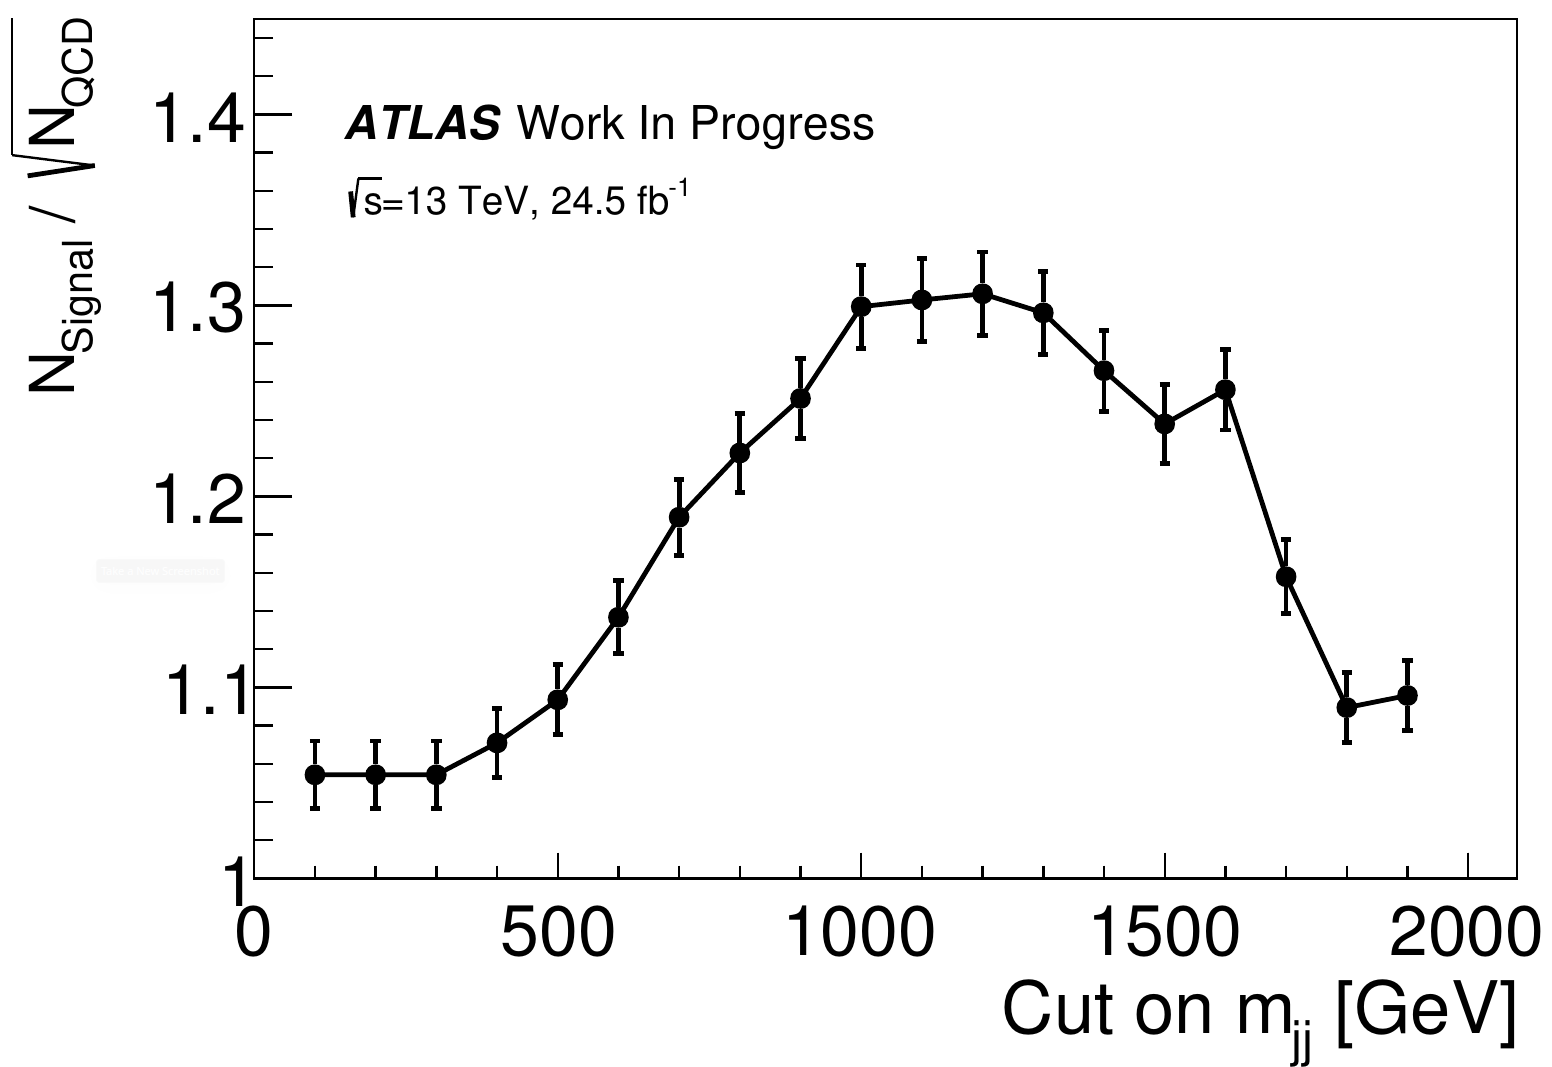
\includegraphics[width=0.5\linewidth,height=\textheight,keepaspectratio]{selection/mjj_significance}
            }
            \subfloat[$\deta_{jj}$ Cut Significance]{
                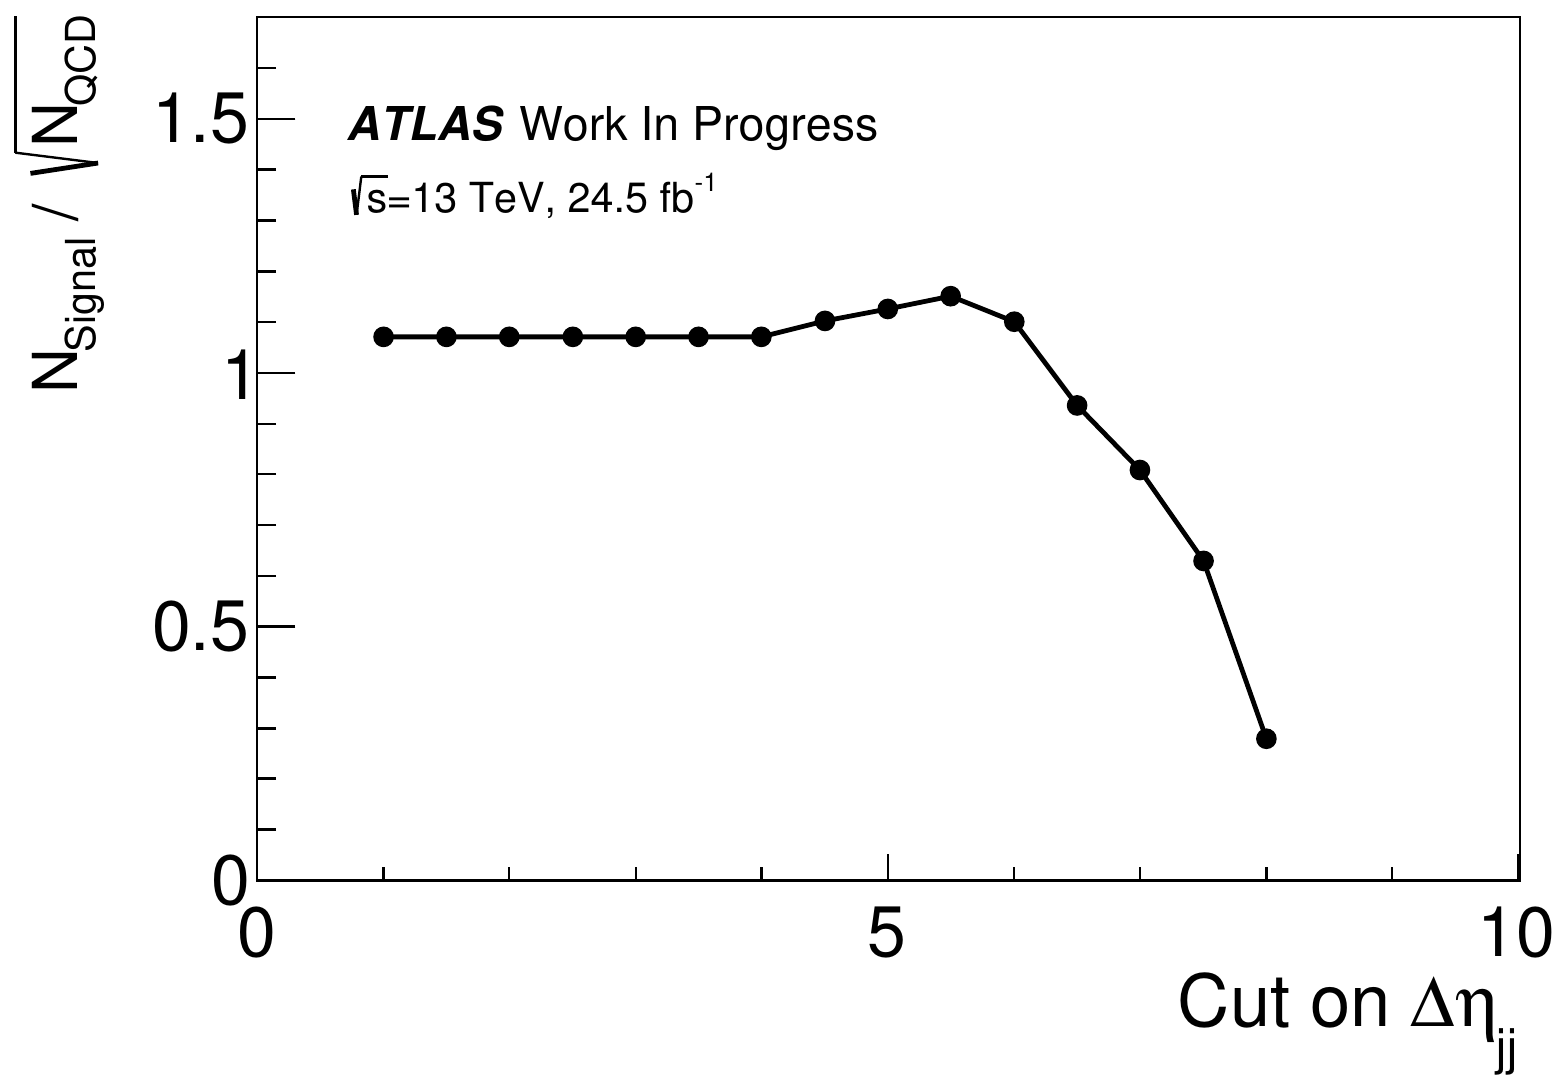
\includegraphics[width=0.5\linewidth,height=\textheight,keepaspectratio]{selection/detajj_significance}
            }\\
            \subfloat[6-Jet Vector-Sum $p_{T}$ Cut Significance]{
                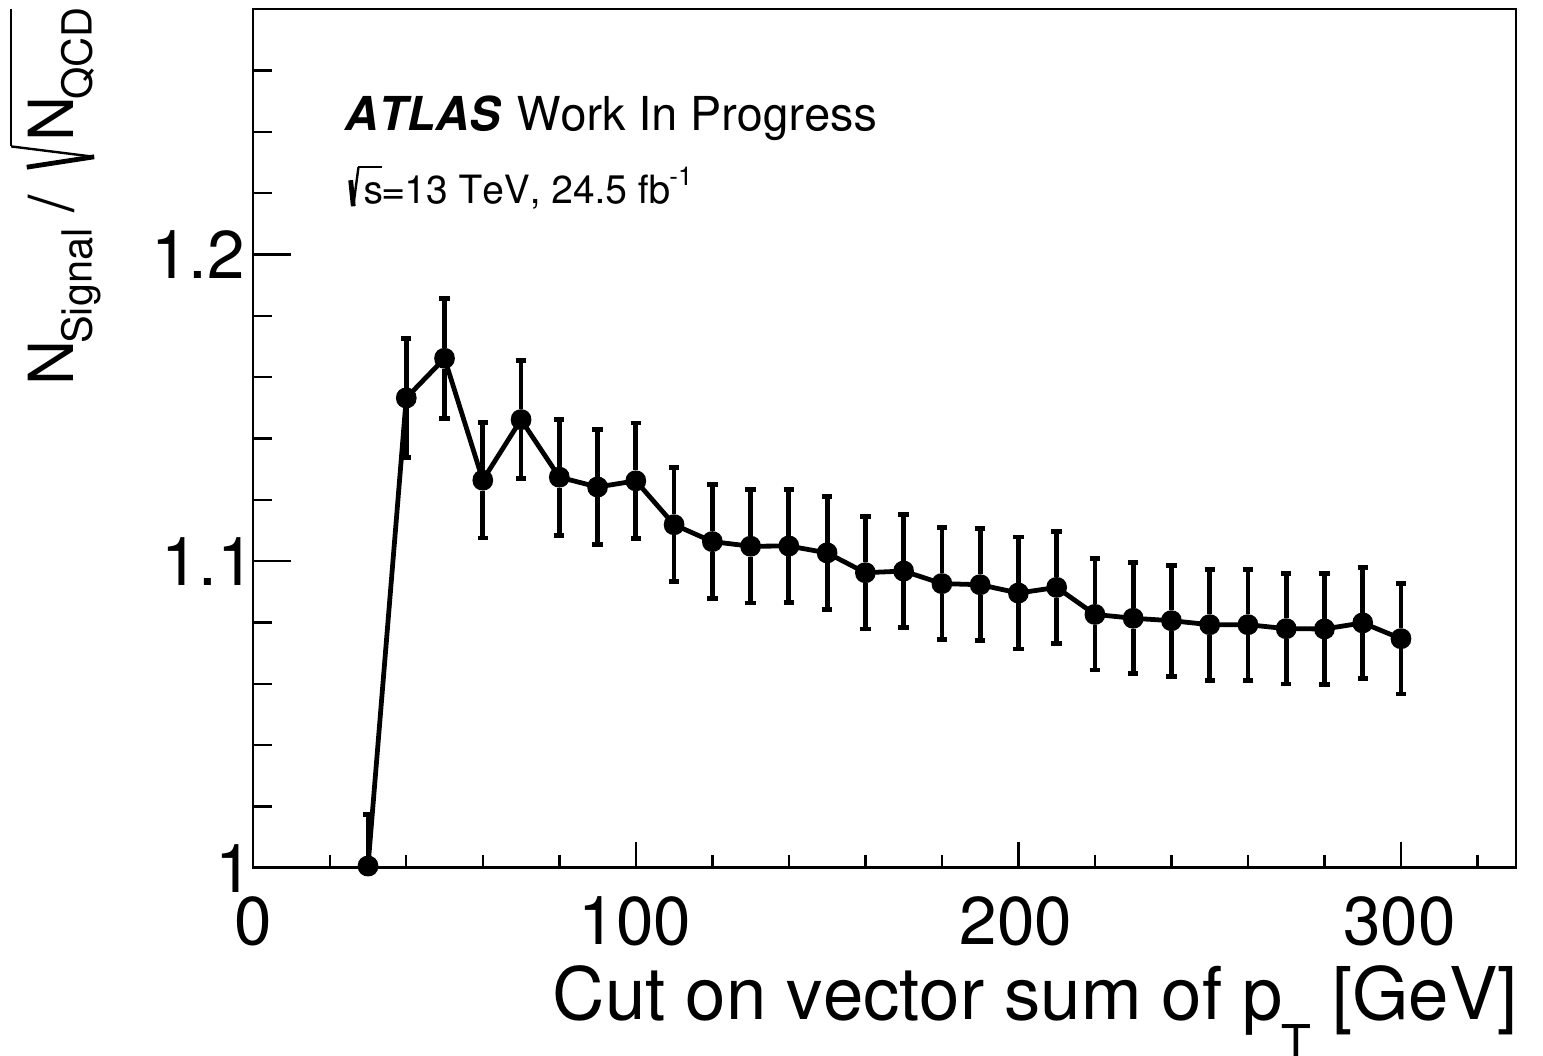
\includegraphics[width=0.5\linewidth,height=\textheight,keepaspectratio]{selection/vecsum_pt}
            }
            \caption{
                Significance value (see Chapter \ref{chapter:results})
                    for different cut values on the various VBF selection criteria\cite{vbf_hh_4b_2018_int}.
                TODO: I might need to replace these (especially the detajj one... that or our current cuts are super wrong).
            }
            \label{fig:vbf_cuts}
        \end{figure}
        \FloatBarrier


    \subsection{B-Quark Pairing}
        
        What is detected within ATLAS and reconstructed by Athena are not Higgs Bosons, but rather their decay products.
        To reconstruct the two Higgs Bosons, the four reconstructed b-quarks must be combined together, two b's to each Higgs.
        A pairing algorithm, called MinDR \cite{hh4b_2021_int_note},
            is used to determine which b-quarks should be paired to each other.
        MinDR operates under the assumption that the decay products of the Higgs boson
            should be relatively close to each other in angular space, maintaining the Higgs' high $p_T$.
        With four jets, which need to be split into two pairs, there are three ways to choose the pairings.
        For each of the three pairing options, MinDR takes the pair with the leading $p_T$ as the ``leading Higgs Candidate''
        The pairing option which is chosen is that which minimizes the $\Delta R$ between the leading Higgs Candidate decay products
            (see Figure \ref{fig:minDR_pairing_diagram}).
        The effectiveness of this algorithm has been validated for multiple values of \kvv and \kl,
            as shown in Figure \ref{fig:HHpairing}.

        \begin{figure}[tbh]
            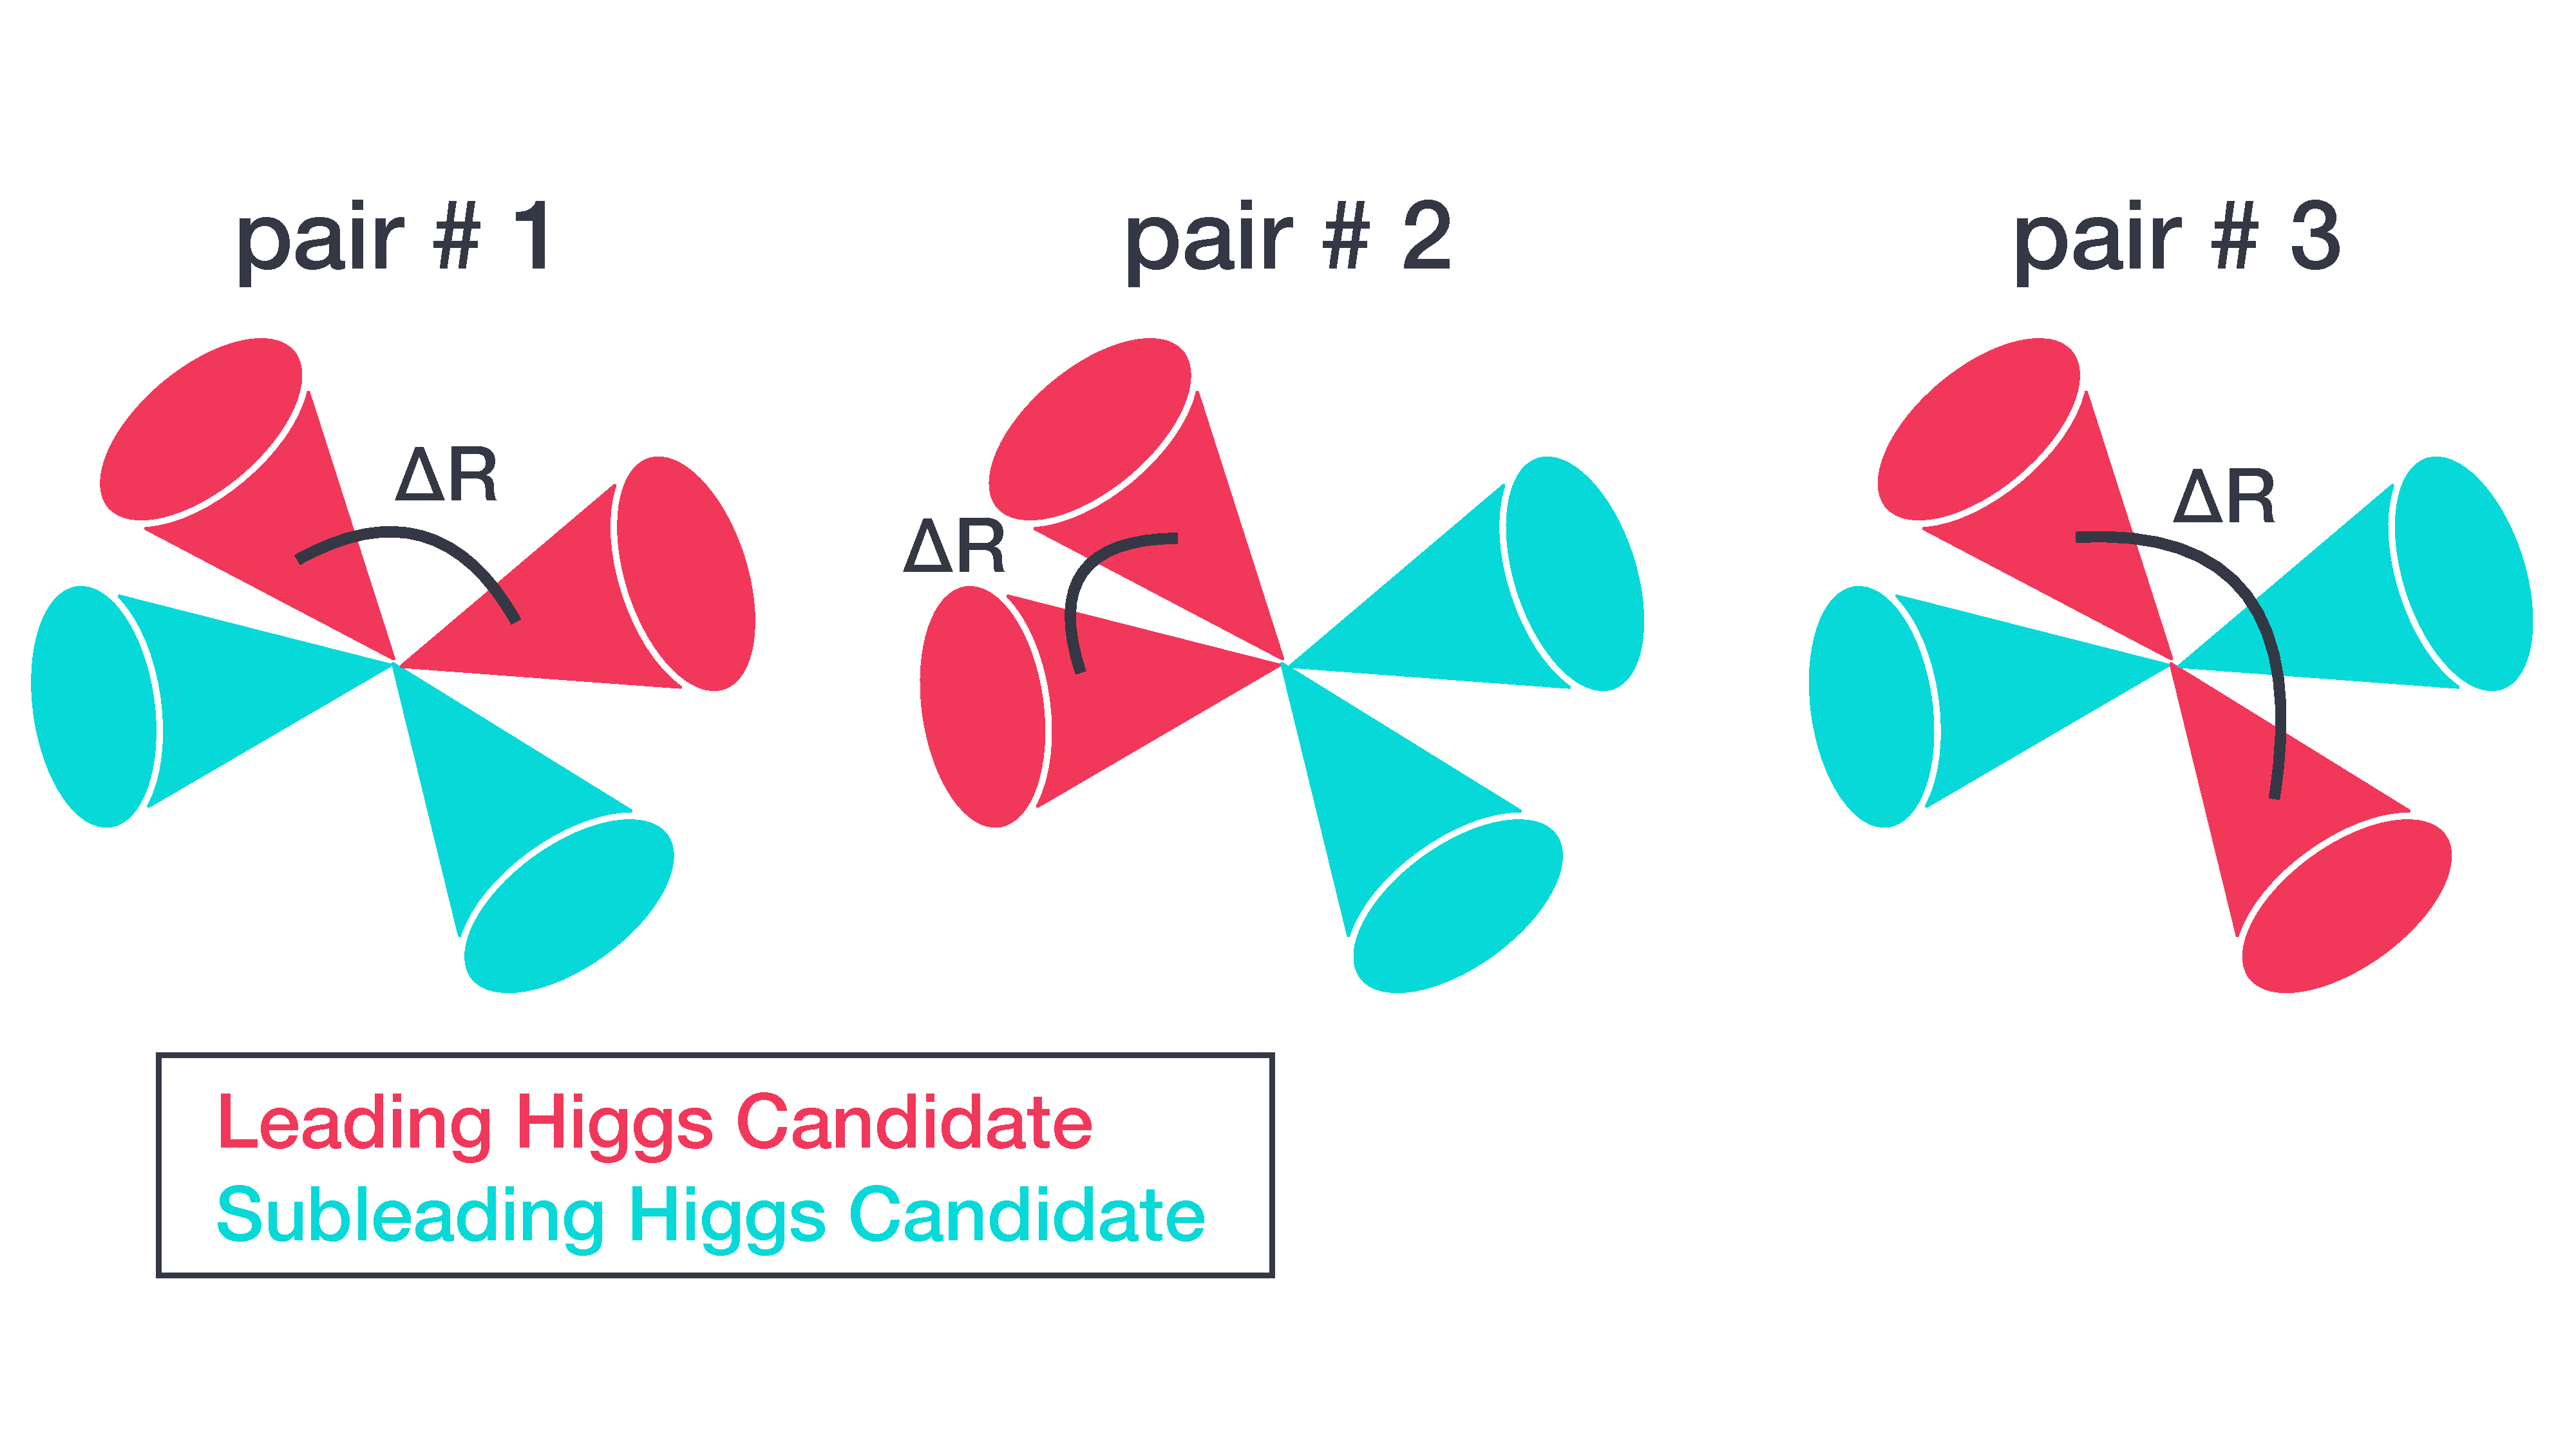
\includegraphics[width=\linewidth,height=\textheight,keepaspectratio]{selection/pairing}
            \caption{
                TODO (minDR picks pair 2 btw)\cite{hh4b_2021_int_note}
            }
            \label{fig:minDR_pairing_diagram}
        \end{figure}

        \begin{figure}[hbt]
            \centering
            \subfloat[Pairing accuracy vs \kl]{
                     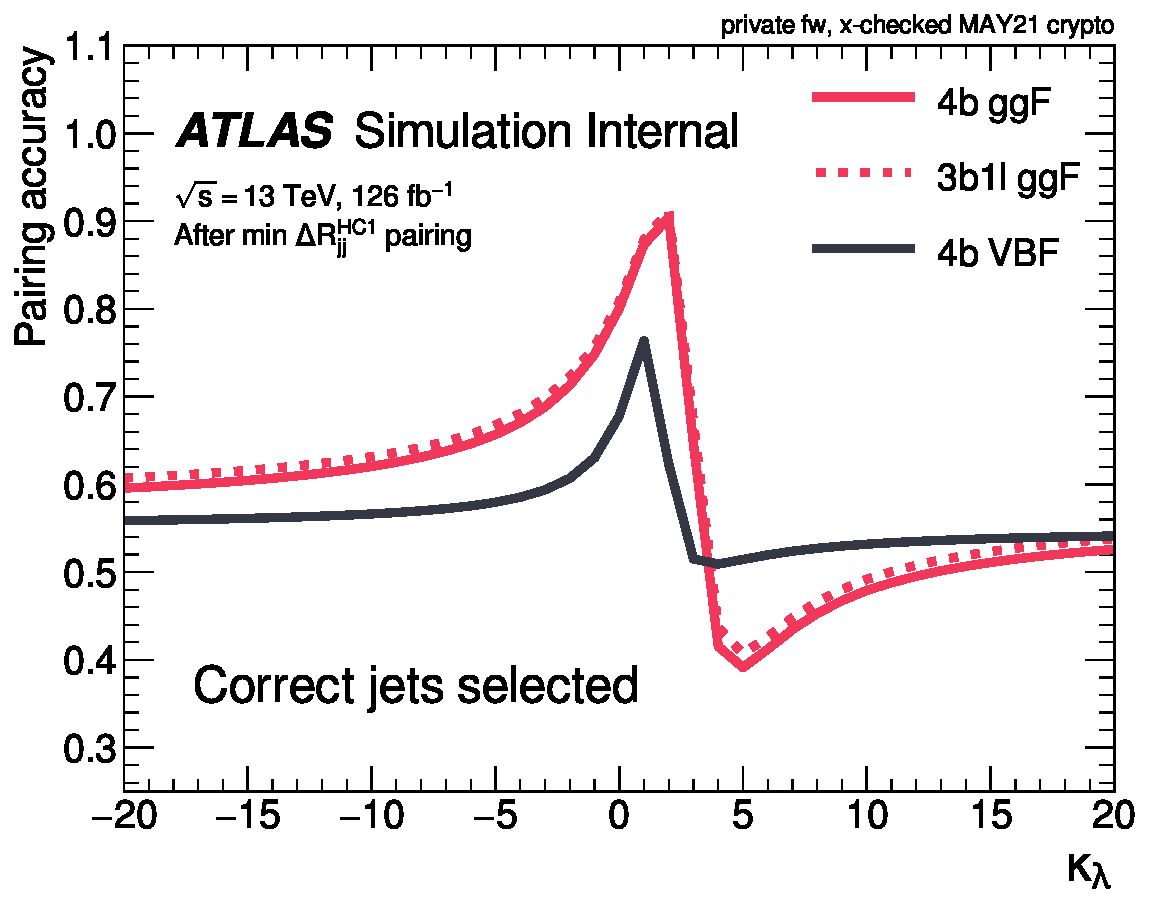
\includegraphics[width=0.4\textwidth]{selection/pairing_accuracy_kl}
                \label{fig:acc_kl_exists}
            }
            \subfloat[Pairing accuracy vs $\kappa_{2V}$]{
                     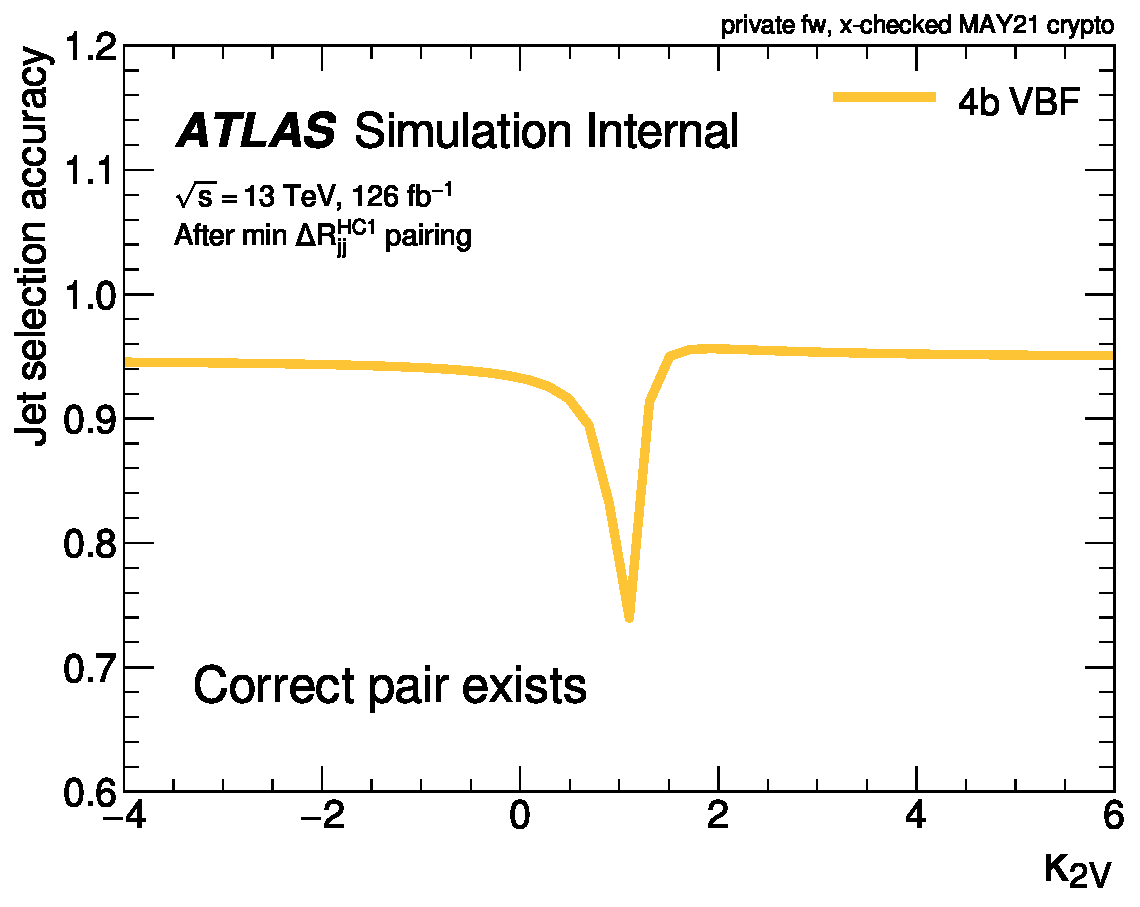
\includegraphics[width=0.4\textwidth]{selection/pairing_accuracy_k2v}
                \label{fig:acc_k2v_exists}
            }
            \caption{TODO \cite{hh4b_2021_int_note}}
            \label{fig:HHpairing}
        \end{figure}
                                                                                                         
        \FloatBarrier


    \subsection{Region Definition}
        
        There are three ``regions'' which are used for the analysis.
        The ``Control'' and ``Validation'' regions are used for the Background Estimation (see Chapter \ref{chapter:background}).
        The ``Signal'' Region is the set of data which will be used to search for the di-Higgs signal.

        The region which an event falls into is based on the reconstructed masses of the leading and sub-leading Higgs.
        The Signal Region (SR) corresponds to those events for which the reconstructed Higgs masses
            align closely with the measured value of the Higgs Boson (125 GeV), with additional room provided for error in measurment.
        The Control and Validation Regions (CR and VR) are adjacent to the Signal Region,
            designating events with kinematics very similar to the Signal Region,
            but with reconstructed Higgs masses incompatible with experimental measurment (see Figure \ref{fig:region_definition}).
        The boundaries of these regions are governed by a quantity $X_HH$, defined as:

        \begin{equation}
            X_{HH} \equiv \sqrt{\left(\frac{m_{H1} - 124\textrm{GeV}}{0.1 \ m_{H1}}\right)^{2}
                + \left(\frac{m_{H2} - 117\textrm{GeV}}{0.1 \ m_{H2}}\right)^{2}}
            \label{eq:xhh}
        \end{equation}
        
        The SR is defined by $X_{hh} < 1.6$,
            while the CR and VR are set within a ring-like shape between the Signal Region
            and an outer bondary defined by:
        \begin{equation}
            \text{CR\ Outer\ Edge} \quad : \quad \sqrt{ \left(m_{H1} - 1.05 \cdot 124\textrm{GeV}\right)^2
                +  \left(m_{H2} - 1.05 \cdot 117\textrm{GeV}\right)^2 } = 45\textrm{GeV}
            \label{eq:cr_out}
        \end{equation}
        
        The split between the CR and VR is based on studies demonstrating that this split results in
            close kinematic similarity between the two regions.

        \begin{figure}[tbh]
            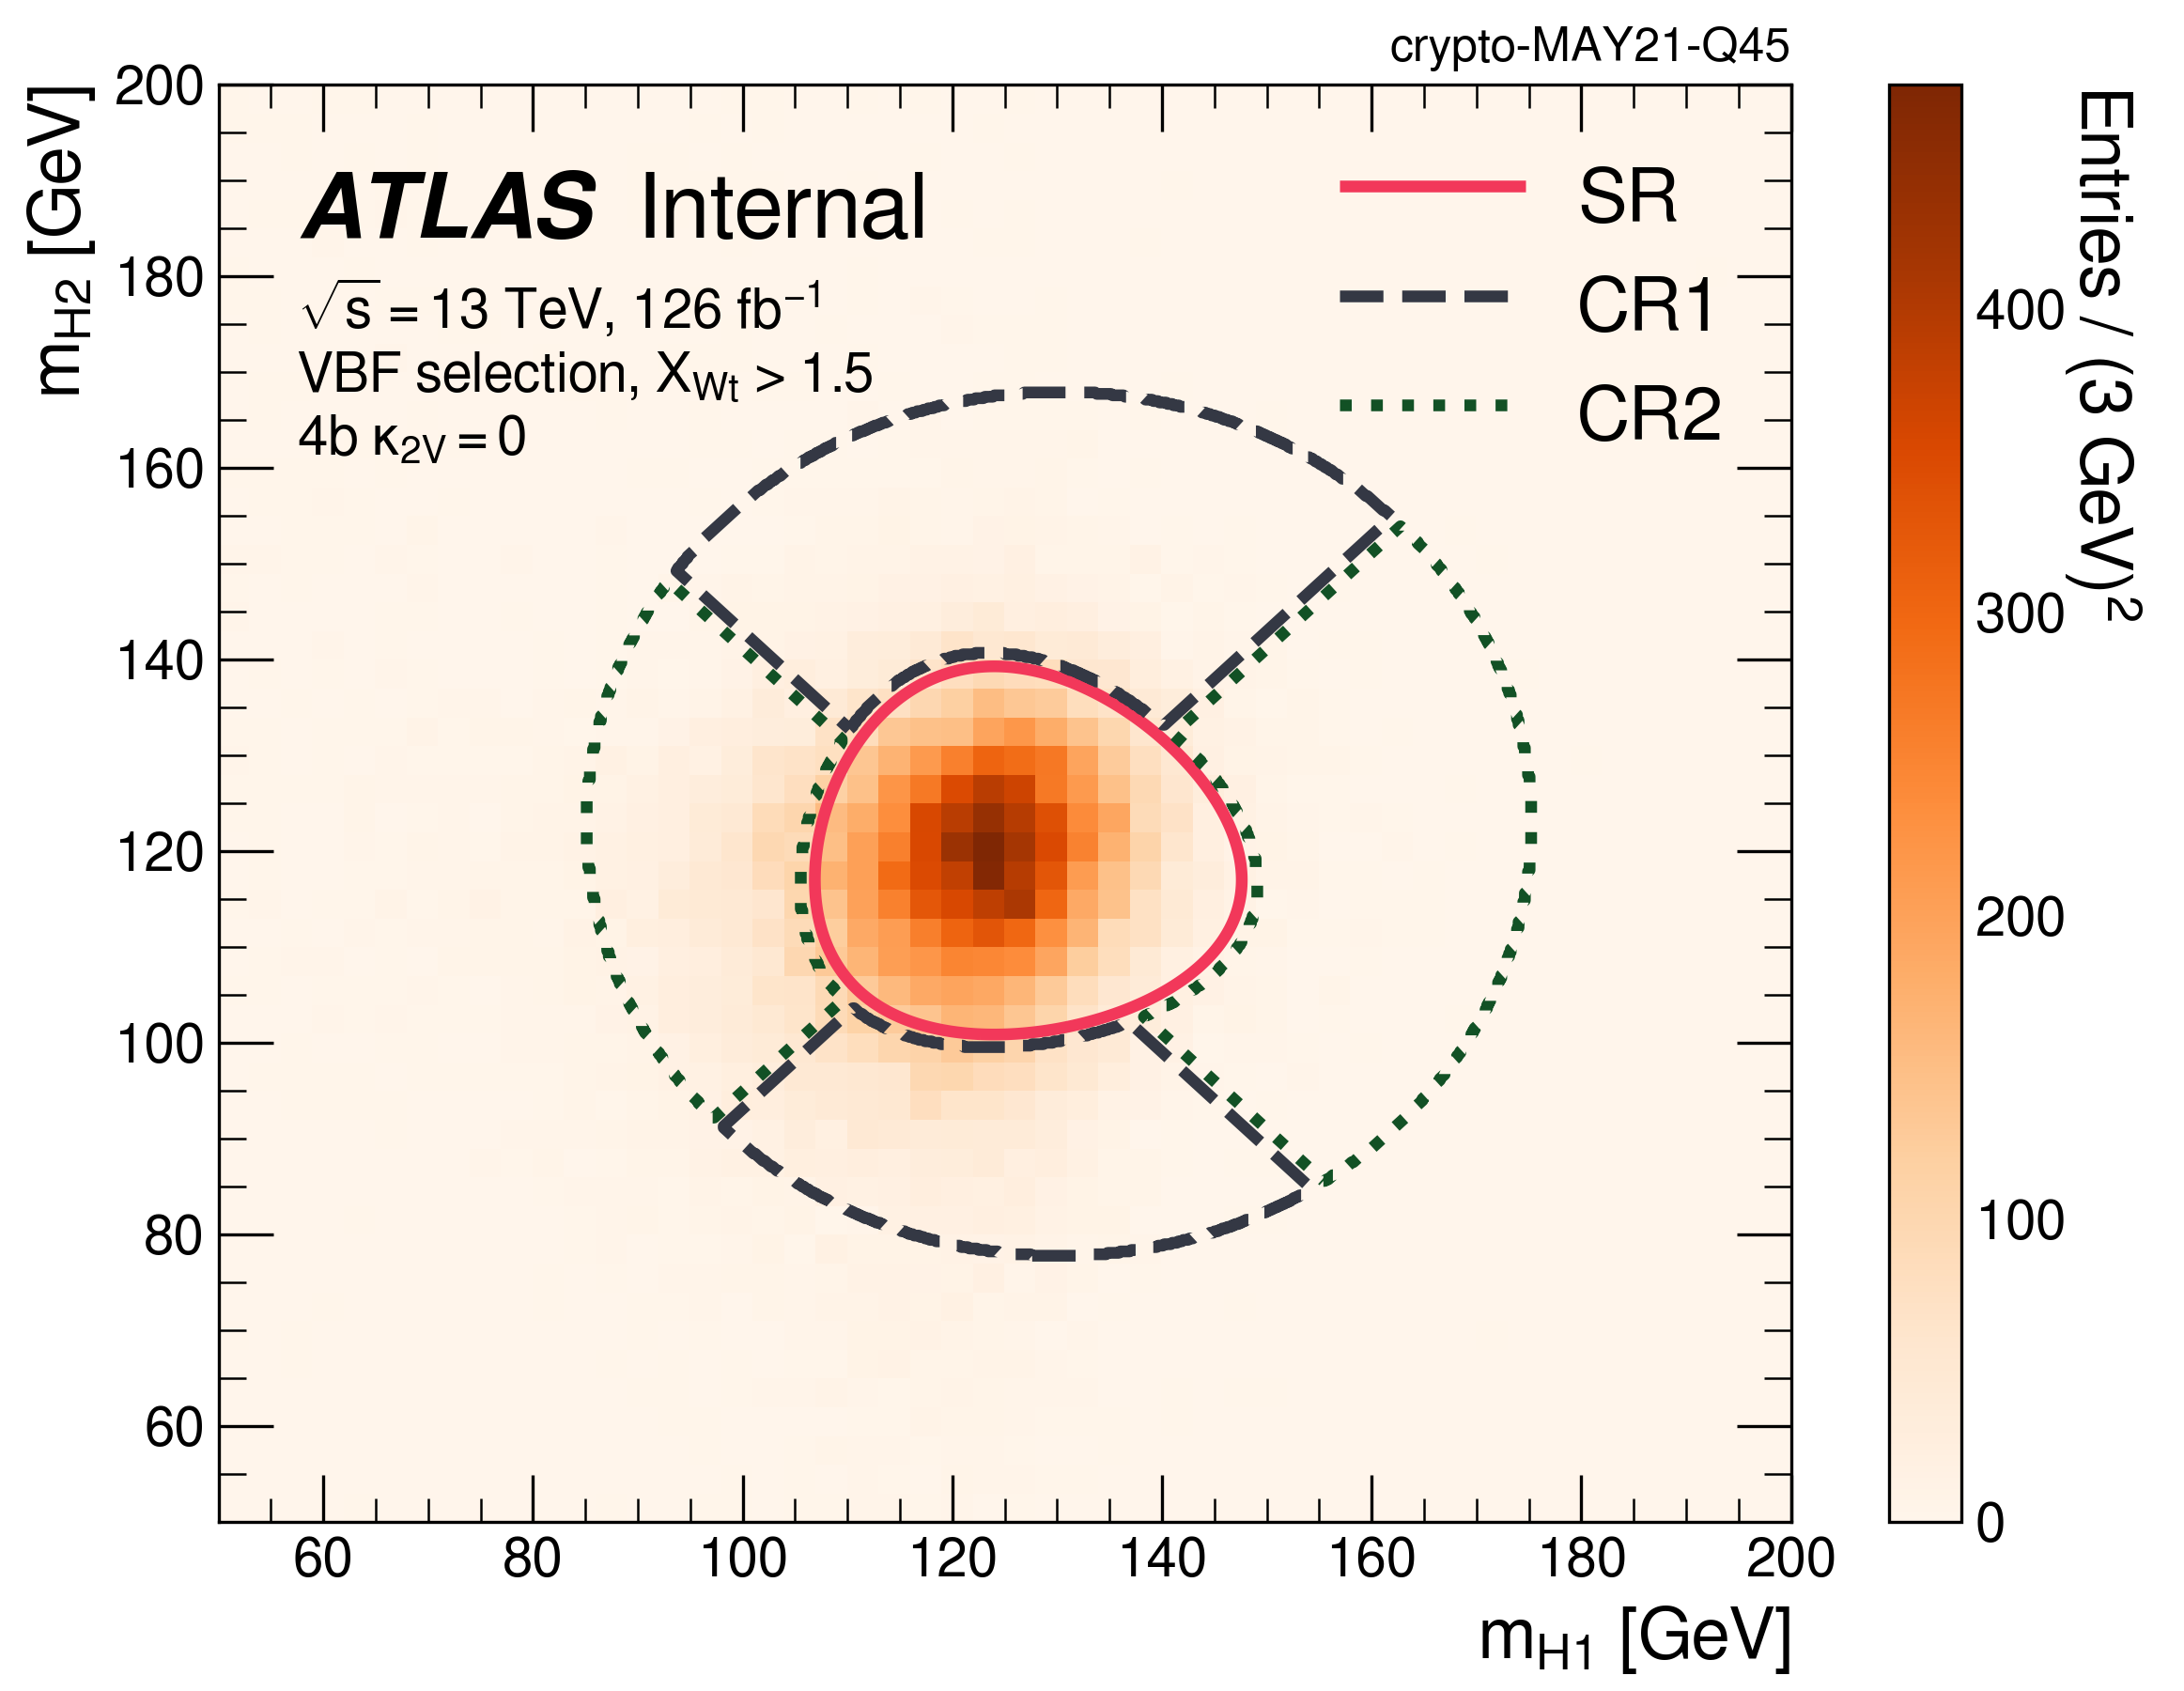
\includegraphics[width=\linewidth,height=\textheight,keepaspectratio]{selection/massplane_sig_all_4b_vbf_Xwt_1.5_k2V_0}
            \caption{
                We use k2v=0 because we're trying to exclude it.\cite{hh4b_2021_int_note}
            }
            \label{fig:region_definition}
        \end{figure}


        %Do I need to show proof of all our cut steps? Like, surely there's a motivation for each of them?

  %      Two VBF Initial Scatter (IS) quark jets:
  %          light jets (u,d, or maybe charm);
  %          high pt;
  %          wide opening angle;
  %          high mjj;
  %          can be central or forward.

  %      Four b-jets:
  %          decay products of higgss;
  %          all central; why are interesting things always central?
  %                       can i show this mathematically (dude it's just Newton's first law... don't overthink it)
  %          also high pt;
  %          b/b-bar products are expected to have very low opening angle between them.

  %      Overall:
  %          Zero pt initially, so expected low pt for vector sum of all jets combined
  %          

  %      Make note of the fact that the anti-$k_t$ algorithm is set with $\Delta R = 0.4$.

  %  kinematic cuts
  %      basic jet multiplicity reqs,
  %      btag jets with DL1r 77\% working point,
  %      4b-tagged, central
  %      also 2b and 3b1f, which are reserved for background estimation
  %      2 non-btagged jets with min-mjj for VBF

  %  Then there's the minDR pairing of b's to reconstruct HH

  %  Then cut on dihiggs and full system kinematics

  %  Then make sure the higgss fall within the "signal region" (their individual masses are approximately 125 GeV)


%...and how we wittle the abundance of events down to a manageable subset.
%If I stick to this format, there's still a bit of event reconstruction done here.
%
%HH4b Resolved Reco and Selection (literally just go through resolved recon...).
%    Final stage is the signal region selection
